\documentclass[a4paper,12pt,twoside]{memoir}

% Castellano
\usepackage[spanish,es-tabla]{babel}
\selectlanguage{spanish}
\usepackage[utf8]{inputenc}
\usepackage[T1]{fontenc}
\usepackage{lmodern} % scalable font
\usepackage{microtype}
\usepackage{placeins}

\RequirePackage{booktabs}
\RequirePackage[table]{xcolor}
\RequirePackage{xtab}
\RequirePackage{multirow}

% Links
\PassOptionsToPackage{hyphens}{url}\usepackage[colorlinks]{hyperref}
\let\oldhref\href
\renewcommand{\href}[2]{\oldhref{#1}{#2}\footnote{\url{#1}}}
\hypersetup{
	allcolors = {red}
}

% Ecuaciones
\usepackage{amsmath}

% Rutas de fichero / paquete
\newcommand{\ruta}[1]{{\sffamily #1}}

% Párrafos
\nonzeroparskip

% Huérfanas y viudas
\widowpenalty100000
\clubpenalty100000

% Evitar solapes en el header
\nouppercaseheads

% Imagenes
\usepackage{graphicx}
\newcommand{\imagen}[2]{
	\begin{figure}[!h]
		\centering
		\includegraphics[width=0.9\textwidth]{#1}
		\caption{#2}\label{fig:#1}
	\end{figure}
	\FloatBarrier
}

\newcommand{\imagenflotante}[2]{
	\begin{figure}%[!h]
		\centering
		\includegraphics[width=0.9\textwidth]{#1}
		\caption{#2}\label{fig:#1}
	\end{figure}
}



% El comando \figura nos permite insertar figuras comodamente, y utilizando
% siempre el mismo formato. Los parametros son:
% 1 -> Porcentaje del ancho de página que ocupará la figura (de 0 a 1)
% 2 --> Fichero de la imagen
% 3 --> Texto a pie de imagen
% 4 --> Etiqueta (label) para referencias
% 5 --> Opciones que queramos pasarle al \includegraphics
% 6 --> Opciones de posicionamiento a pasarle a \begin{figure}
\newcommand{\figuraConPosicion}[6]{%
	\setlength{\anchoFloat}{#1\textwidth}%
	\addtolength{\anchoFloat}{-4\fboxsep}%
	\setlength{\anchoFigura}{\anchoFloat}%
	\begin{figure}[#6]
		\begin{center}%
			\Ovalbox{%
				\begin{minipage}{\anchoFloat}%
					\begin{center}%
						\includegraphics[width=\anchoFigura,#5]{#2}%
						\caption{#3}%
						\label{#4}%
					\end{center}%
				\end{minipage}
			}%
		\end{center}%
	\end{figure}%
}

%
% Comando para incluir imágenes en formato apaisado (sin marco).
\newcommand{\figuraApaisadaSinMarco}[5]{%
	\begin{figure}%
		\begin{center}%
			\includegraphics[angle=90,height=#1\textheight,#5]{#2}%
			\caption{#3}%
			\label{#4}%
		\end{center}%
	\end{figure}%
}
% Para las tablas
\newcommand{\otoprule}{\midrule [\heavyrulewidth]}
%
% Nuevo comando para tablas pequeñas (menos de una página).
\newcommand{\tablaSmall}[5]{%
	\begin{table}
		\begin{center}
			\rowcolors {2}{gray!35}{}
			\begin{tabular}{#2}
				\toprule
				#4
				\otoprule
				#5
				\bottomrule
			\end{tabular}
			\caption{#1}
			\label{tabla:#3}
		\end{center}
	\end{table}
}

%
%Para el float H de tablaSmallSinColores
\usepackage{float}

%
% Nuevo comando para tablas pequeñas (menos de una página).
\newcommand{\tablaSmallSinColores}[5]{%
	\begin{table}[H]
		\begin{center}
			\begin{tabular}{#2}
				\toprule
				#4
				\otoprule
				#5
				\bottomrule
			\end{tabular}
			\caption{#1}
			\label{tabla:#3}
		\end{center}
	\end{table}
}

\newcommand{\tablaApaisadaSmall}[5]{%
	\begin{landscape}
		\begin{table}
			\begin{center}
				\rowcolors {2}{gray!35}{}
				\begin{tabular}{#2}
					\toprule
					#4
					\otoprule
					#5
					\bottomrule
				\end{tabular}
				\caption{#1}
				\label{tabla:#3}
			\end{center}
		\end{table}
	\end{landscape}
}

%
% Nuevo comando para tablas grandes con cabecera y filas alternas coloreadas en gris.
\newcommand{\tabla}[6]{%
	\begin{center}
		\tablefirsthead{
			\toprule
			#5
			\otoprule
		}
		\tablehead{
			\multicolumn{#3}{l}{\small\sl continúa desde la página anterior}\\
			\toprule
			#5
			\otoprule
		}
		\tabletail{
			\hline
			\multicolumn{#3}{r}{\small\sl continúa en la página siguiente}\\
		}
		\tablelasttail{
			\hline
		}
		\bottomcaption{#1}
		\rowcolors {2}{gray!35}{}
		\begin{xtabular}{#2}
			#6
			\bottomrule
		\end{xtabular}
		\label{tabla:#4}
	\end{center}
}

%
% Nuevo comando para tablas grandes con cabecera.
\newcommand{\tablaSinColores}[6]{%
	\begin{center}
		\tablefirsthead{
			\toprule
			#5
			\otoprule
		}
		\tablehead{
			\multicolumn{#3}{l}{\small\sl continúa desde la página anterior}\\
			\toprule
			#5
			\otoprule
		}
		\tabletail{
			\hline
			\multicolumn{#3}{r}{\small\sl continúa en la página siguiente}\\
		}
		\tablelasttail{
			\hline
		}
		\bottomcaption{#1}
		\begin{xtabular}{#2}
			#6
			\bottomrule
		\end{xtabular}
		\label{tabla:#4}
	\end{center}
}

%
% Nuevo comando para tablas grandes sin cabecera.
\newcommand{\tablaSinCabecera}[5]{%
	\begin{center}
		\tablefirsthead{
			\toprule
		}
		\tablehead{
			\multicolumn{#3}{l}{\small\sl continúa desde la página anterior}\\
			\hline
		}
		\tabletail{
			\hline
			\multicolumn{#3}{r}{\small\sl continúa en la página siguiente}\\
		}
		\tablelasttail{
			\hline
		}
		\bottomcaption{#1}
		\begin{xtabular}{#2}
			#5
			\bottomrule
		\end{xtabular}
		\label{tabla:#4}
	\end{center}
}



\definecolor{cgoLight}{HTML}{EEEEEE}
\definecolor{cgoExtralight}{HTML}{FFFFFF}

%
% Nuevo comando para tablas grandes sin cabecera.
\newcommand{\tablaSinCabeceraConBandas}[5]{%
	\begin{center}
		\tablefirsthead{
			\toprule
		}
		\tablehead{
			\multicolumn{#3}{l}{\small\sl continúa desde la página anterior}\\
			\hline
		}
		\tabletail{
			\hline
			\multicolumn{#3}{r}{\small\sl continúa en la página siguiente}\\
		}
		\tablelasttail{
			\hline
		}
		\bottomcaption{#1}
		\rowcolors[]{1}{cgoExtralight}{cgoLight}
		
		\begin{xtabular}{#2}
			#5
			\bottomrule
		\end{xtabular}
		\label{tabla:#4}
	\end{center}
}




\graphicspath{ {./img/} }

% Capítulos
\chapterstyle{bianchi}
\newcommand{\capitulo}[2]{
	\setcounter{chapter}{#1}
	\setcounter{section}{0}
	\chapter*{#2}
	\addcontentsline{toc}{chapter}{#2}
	\markboth{#2}{#2}
}

% Apéndices
\renewcommand{\appendixname}{Apéndice}
\renewcommand*\cftappendixname{\appendixname}

\newcommand{\apendice}[1]{
	%\renewcommand{\thechapter}{A}
	\chapter{#1}
}

\renewcommand*\cftappendixname{\appendixname\ }

% Formato de portada
\makeatletter
\usepackage{xcolor}
\newcommand{\tutor}[1]{\def\@tutor{#1}}
\newcommand{\course}[1]{\def\@course{#1}}
\definecolor{cpardoBox}{HTML}{E6E6FF}
\def\maketitle{
	\null
	\thispagestyle{empty}
	% Cabecera ----------------
	\noindent
\includegraphics[width=\textwidth]{cabecera}\vspace{1cm}%
	\vfill
	% Título proyecto y escudo informática ----------------
	\colorbox{cpardoBox}{%
		\begin{minipage}{.8\textwidth}
			\vspace{.5cm}\Large
			\begin{center}
				\textbf{TFG del Grado en Ingeniería Informática}\vspace{.6cm}\\
				\textbf{\LARGE\@title{}}
			\end{center}
			\vspace{.2cm}
		\end{minipage}
		
	}%
	\hfill\begin{minipage}{.20\textwidth}
		
\includegraphics[width=\textwidth]{escudoInfor}
	\end{minipage}
	\vfill
	% Datos de alumno, curso y tutores ------------------
	\begin{center}%
		{%
			\noindent\LARGE
			Presentado por \@author{}\\ 
			en Universidad de Burgos --- \@date{}\\
			\begin{tabbing}
				Tutores: \= Dr. César Ignacio García Osorio \kill
				Tutores: \> Dr. César Ignacio García Osorio \\
				\> Dr. José Francisco Diez Pastor
			\end{tabbing}
		}%
	\end{center}%
	\null
	\cleardoublepage
}
\makeatother


% Datos de portada
\title{Flutter Games\\Documentación Técnica}
\author{Samuel Casal Cantero}
\tutor{José Francisco Diez Pastor y César García Osorio}
\date{\today}

\begin{document}
	
	\maketitle
	
	
	
	\cleardoublepage
	
	%% Comando para mostrar el header de las tablas en negrita
	
	
	
	%%%%%%%%%%%%%%%%%%%%%%%%%%%%%%%%%%%%%%%%%%%%%%%%%%%%%%%%%%%%%%%%%%%%%%%%%%%%%%%%%%%%%%%%
	
	
	
	\frontmatter
	
	
	\clearpage
	
	% Indices
	\tableofcontents
	
	\clearpage
	
	\listoffigures
	
	\clearpage
	
	\listoftables
	
	\clearpage
	
	\mainmatter
	
	\appendix
	
	\apendice{Plan de Proyecto Software}

\section{Introducción}
En este apartado trabajaremos sobre la planificación del proyecto, de tal manera que se pueda definir, identificar y programar las actividades específicas que se requieren para realizar las tareas del mismo. 

La evolución temporal es una de las partes más importantes de todo el proceso de desarollo, ya que una mala planificación, puede hacer que el proyecto sufra retrasos, de tal manera, que no se llegue a la fecha de entrega prevista, lo que supone un coste, en este caso, el suspenso, pero también el económico, por las horas y recursos destinados a tal fin.

 En esta fase es muy importante que para cada una de las tareas sepamos el tiempo que durará aproximadamente, quien es el encargado de hacer la tarea y el dinero que supone hacerla. Por lo que invertir tiempo en la estimación de las horas cada una de las tareas, ayuda a identificar las irregularidades en el futuro.

La viabilidad pone el foco en el coste económico del proyecto como de la parte legal. Es decir, es un reactivo limitante, sobre todo el coste.

\section{Planificación temporal}
El método de trabajo para hacer el seguimiento y la planificación del mismo es Scrum, que pretende realizar una gestión ágil del proyecto. Se basa en \emph{spints}, la duración de estos suele rondar entre los siete y quince días. Dependiendo de los requisitos del proyecto, número de integrantes y del tiempo disponible, se maneja esta horquilla temporal, en mi caso por la falta de tiempo, decidí hacerlos de 5 días. 

Estos \emph{sprints} se basan en una reunión donde se ponen todas las tareas que se tiene como objetivo realizar, en mi caso eran las reuniones con los tutores del trabajo de fin de grado. Además cada día se tiene que hacer el \emph{daily meetting}, pero como el proyecto es unipersonal, no es necesario. Por lo que se puede afirmar que se ha seguido la filosofía ágil.

Todo ello esta integrado en un proceso incremental de desarrollo del producto, ya que en cada uno de los \emph{spirnts} se producen las mejoras planificadas.

Aclarar que la estimación del tiempo se realiza mediante los \emph{story points}, que indican la complejidad de la tarea a realizar. Esta herramienta nos la aporta ZenHub, con la siguiente relación según el coste temporal:

\tablaSmall{Equivalencias \emph{Story Points} y tiempo estimado}{c c }{StoryPoints/tiempo}
{ \multicolumn{1}{l}{Story Points} & Estimación temporal \\}{ 
	1            & 1 hora              \\ 
	2            & 2 horas           \\ 
	3            & 3 horas             \\ 
	4            & 4 horas           \\ 
	5            & 5 horas             \\ 
	6            & 6 horas           \\ 
	7            & 7 horas             \\ 
	8            & 8 horas             \\ 
	9            & 9 horas             \\ 
}

Algo que define mucho la duración de los \emph{sprints} a 5 días, es porque el proyecto en el que estaba, no me funcionaba y al final decidí por hacer este otro. Esto implica tener mayor cantidad de \emph{sprints}, con un incremento del aplicación mayor, ya que el margen temporal hasta la entrega era de un mes. 

A continuación se detallan cada uno de los \emph{sprints} realizados durante el proyecto:

\subsection{Sprint 1 (22/06/20 - 26/096/20)}\label{sprint-1-220620---260620}

El inicio del proyecto fue a través de correo, explicando la situación a mis tutores, de que lo que estaba haciendo no me funcionaba, que estaba verde y que si cabía la posibilidad de hacer otro trabajo. Me dieron el visto bueno, pero que tenía que hacer algo diferenciador, ya que no vale cualquier cosa. Por lo que en la reunión de cierre de \emph{sprint} se comentaría como centrar la aplicación. 

Entonces debido a la escasez temporal, me decido a hacer una aplicación en \emph{Flutter}, ya que se puede hacer algo de calidad de manera ágil.

Los objetivos en este \emph{sprint} inicial fueron:

\begin{itemize}
\item Documentar como hacer aplicaciones en \emph{Flutter}.
\item Cursar un curso en \href{https://www.udemy.com/course/flutter-primeros-pasos/}{Udemy}
\item Crear el repositorio.
\item Implementar el cuerpo de la aplicación.
\item Investigar sobre \emph{apis} que ofrece el \emph{framework}.
\end{itemize}

Todas las \emph{issues} realizadas para este \emph{sprint}, están disponibles en \href{https://github.com/scc0034/flutter_serpiente/milestone/1?closed=1}{Sprint 1}

La estimación fue de 54 horas, pero que finalmente se destinaron 45,5 horas, debido en gran parte a la reutilización de código del curso, aunque el curso me duró más de lo estimado.

\imagen{burndowns/sp1.png}{Sprint 1.}


\section{Estudio de viabilidad}

\subsection{Viabilidad económica}

\subsection{Viabilidad legal}



	\apendice{Especificación de Requisitos}

\section{Introducción}

\section{Objetivos generales}

\section{Catalogo de requisitos}

\section{Especificación de requisitos}



	\apendice{Especificación de diseño}

\section{Introducción}\label{diseño}
En este apéndice se recoge el diseño de las interfaces, como se resolvieron los requisitos funcionales anteriormente expuestos~\pageref{requisitos}, el manejo de los datos o la estructura de los mismos.

\section{Diseño de datos}
En el tratamiento de los datos, se ha optado por hacerlo de dos formas diferentes, esto es debido, a que se necesita persistencia local y externa. Dependiendo de eso, tenemos dos diseños de datos diferentes.

\begin{itemize}
	\item \textbf{FireStore:} es la base de datos integrada en Firestore. Esta no sigue el modelo clásico, ya que es noSQL~\cite{wiki:nosql}, es decir, al igual que mongoDB~\cite{wiki:mongodb}, esta se gestiona mediante ficheros \emph{.json}. A diferencia SGBDR (Sistema gestor de bases de datos relacionales), la manera de trabajar de Firestore, es mediante un modelos no relacionales. Esta fue usada para la persistencia externa de datos. Como se puede ver en la siguiente imagen~\ref{fig:firestore} de la consola de Firebase:
	
	\begin{figure}[H]
		\centering
		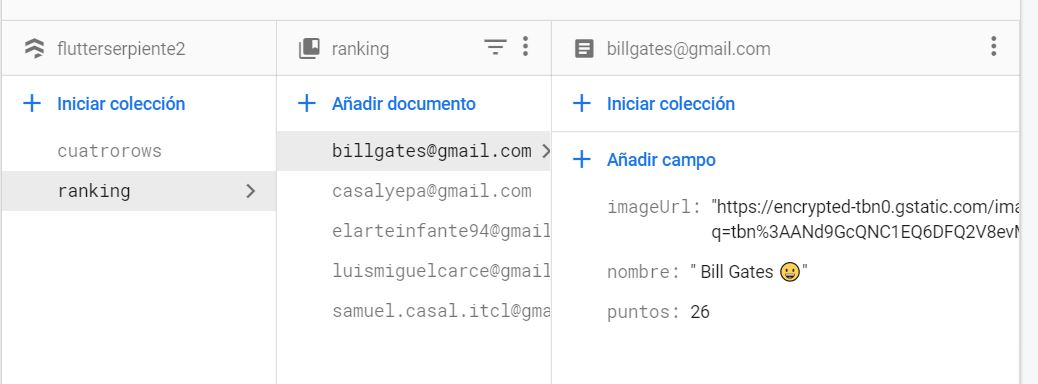
\includegraphics[width=0.9\textwidth]{disenio/firestore.jpg}
		\caption{Base de datos en firestore}\label{fig:firestore}
	\end{figure}

	\item\label{sqlflite} \textbf{Sqlflite:} esta base de datos si que sigue el modelo tradicional del SGBDR. En mi caso fue necesario usar este paquete~\cite{package:sqlflite}, que internamente funciona con sqlite. Usado para almacenar datos en forma local, ya que no era necesario que los datos salieran del terminal. Una de las cosas a tener en cuenta de esto, es que si el usuario borra la caché de la aplicación o la desinstala se borran los ficheros correspondientes. Esto no debe de ser problema, ya que solo queremos almacenar ciertos valores.
	
\end{itemize}

\subsection{Diagrama entidad relación}
\begin{itemize}
	\item \textbf{FireStore:} la distribución en la base de datos es mediante colecciones, ver imagen~\ref{fig:diagramfirestore}. Como ejemplo podemos tener la colección para almacenar los datos del ranking, y para cada una de las entradas del ranking un fichero \emph{.josn} que haga referencia a los datos de cada usuario. Aunque esta no siga el modelo relacional, si que se podría implementar un diagrama entidad-relación, pero no se hace, porque es similar a tener dos tablas (colecciones en este caso) en la base de datos y que no tiene relación entre sí.
	
	\begin{figure}[H]
		\centering
		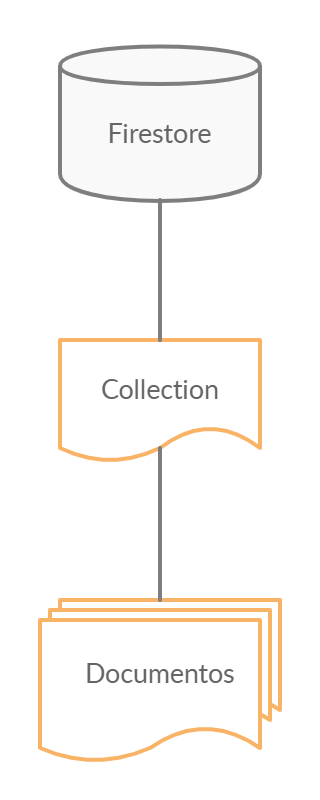
\includegraphics[height=0.9\textwidth]{disenio/diagramafirestore.jpg}
		\caption{Diagrama BD firestore}\label{fig:diagramfirestore}
	\end{figure}

	Una vez sabemos como es el funcionamiento de la base de datos noSQL, las dos colecciones necesarias para la aplicación fueron:
	
	\begin{itemize}
		\item \textbf{ranking:} se encarga de almacenar la mejor puntuación de cada uno de los jugadores del snake~\ref{fig:rankingexample}. Para distinguir cada uno de los documentos, se usa como clave primaria el correo del usuario, que también será el nombre que identifique a cada uno de estos ficheros.
		
		Las variables que almacena son: nombre(String), imagenUrl(String) y puntuación(int). 
		
		\begin{figure}[H]
			\centering
			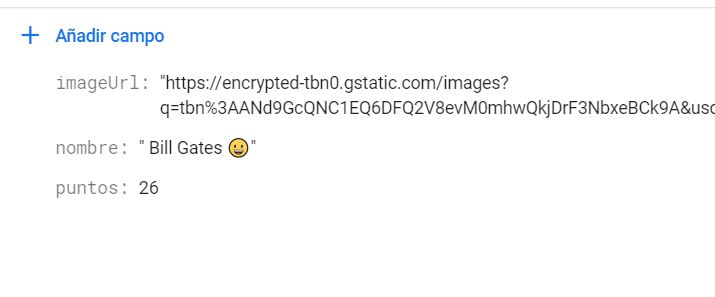
\includegraphics[width=0.9\textwidth]{disenio/rankingexample.jpg}
			\caption{Contenido json de rankinig}\label{fig:rankingexample}
		\end{figure}
	
		\item \textbf{cuatrorows:} esta colección guarda cada una de las partidas online del juego cuatro en raya~\ref{fig:cuatrorowsexample}. Los nombres de los documentos se generan de manera única en la base de datos, por lo que no puede haber dos partidas iguales.
		
		Por lo que la \emph{key} compartida durante el juego es la misma que el nombre del documento, dentro de esta colección. Los campos que tiene este documentos son muchos y variados, pero los más destacados son: 
		
		\begin{itemize}
			\item Posición de cada una de las fichas, de tipo String, y los valores que toma son Y, R o \emph{null}, dependiendo de la ficha que se encuentre en la celda.
			\item Datos de los jugadores, tanto como para el que crea la partida como el que recibe la invitación, estos son: nombre, imagenUrl, correos ... Todos de tipo String.
			\item Flags para controlar si se producen ciertos eventos, como puede ser el final de la partida, si se ha mostrado el mensaje, lanzamiento de la moneda para el sorteo de quien inicia o el mensaje escrito por cada uno de los jugadores. Todas ellas son de tipo String, exceptuando las que puedan tomar valores de verdadero o falso.
		\end{itemize}
	
		\begin{figure}[H]
			\centering
			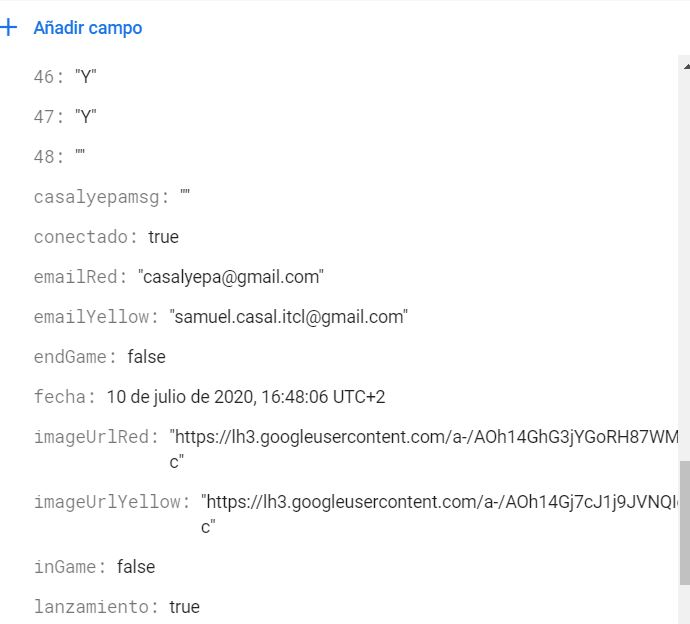
\includegraphics[width=0.9\textwidth]{disenio/cuatrorowsexample.jpg}
			\caption{Contenido json de cuatorows}\label{fig:cuatrorowsexample}
		\end{figure}
	\end{itemize}
	
	\item \textbf{Sqlflite:} usada para la persistencia interna de datos. No tiene diagrama de entidad relación ya que solo consta de una tabla. Como se puede ver en la imagen~\ref{fig:tablasqlflite}, este método se encarga de crear el recurso de la tabla, en el caso de que no existan, (cuando se instala la aplicación en el terminal).
	
	\begin{figure}[H]
		\centering
		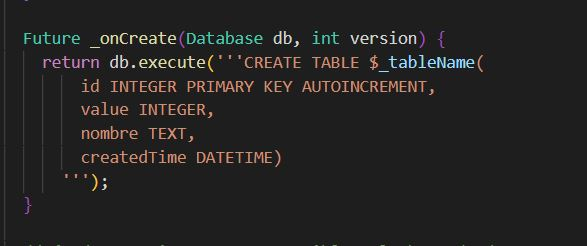
\includegraphics[width=0.9\textwidth]{disenio/tablasqlflite.png}
		\caption{Método para crear la tabla en la base de datos local}\label{fig:tablasqlflite}
	\end{figure}

	Cada uno de los campos de esta tabla significan:
	\begin{itemize}
		\item \textbf{id:} identificador de tipo entero autoincrementable. Se usa internamente nada más, al final estas variables que almacena, se van a identificar por el nombre.
		\item \textbf{value:} valor que toma esta variable de tipo entero, puede ser 0 o 1, para las de tipo \emph{bool} o valores numéricos. Se hace así con el fin de abarcar estos dos tipos de datos.
		\item \textbf{nombre:} es de tipo String, usada para reconocer a cada una de las variables en la tabla.
		\item \textbf{createdTime:} fecha en la que se añade a la tabla una nueva variable. El tipo de dato que almacena es \emph{datetime}.
	\end{itemize}

	Un ejemplo de uso, lo podemos encontrar dentro de la aplicación en el apartado de \emph{settings}, donde cada vez que se cambia el valor de un \emph{slider} se actualiza en la base de datos. Esto se hace para que cuando el usuario vuelva a la aplicación, la configuración de la última vez que estuvo se siga manteniendo.
	
\end{itemize}

Otra de las formas en las que se almacenan los datos es mediante un fichero en local. Esto solo es usado para la configuración del menú, ya que cada vez que se crea el \emph{Widget} del menú lateral, lee el \emph{.json} para sacar los datos necesarios. Esta lógica de negocio se podría haber usado de la misma forma para solventar el problema de sqlflite~\pageref{sqlflite}.

\section{Diseño procedimental}
Para la gran mayoría de procesos importantes se han hecho diagramas de flujo, con el fin de resolver y comprender algunas de las lógicas de negocio más importantes. Como puede ser el siguiente diagrama~\ref{fig:snakediagrama} para la partida del snake:

%%%%%%%%%%%%%%%%%%%%%%%%%%%%%%%%%%%%%%%%%%%%%%%%%%%%%%%%%SARA

\section{Diseño arquitectónico}
La arquitectura de la aplicación ha seguido el el patrón de diseño BLoC~\cite{xurxodev:bloc}. Significa \emph{Business Logic Component}. Fue creado por Paolo Soare y Cong Hu, los dos de Google y presentado en la conferencia de Dart en 2018. Por lo que es algo bastante nuevo.

Para comprender el porque de esta arquitectura es necesario saber como funcionan los estados compartidos entre los componentes en los framework declarativos~\pageref{declarativo}.

\subsection{Framework declarativo}\label{declarativo}
Los framework declarativos son aquellos donde las vistas se crean y actualizan en base a los datos con los que la vista esta enlazada, de tal forma que, cuando estos datos cambian de valor, se actualizan con una nueva renderización.



	\apendice{Documentación técnica de programación}

%%INTRODUCCION
\section{Introducción}
En este anexo se describe la documentación técnica de programación para este proyecto. Incluye los primeros pasos que son la instalación del proyecto, la estructura de la aplicación o finalmente como compilarlo, desplegarlo o los diferentes tipos de configuraciones realizados. La idea es poder facilitar a los futuros desarrolladores una guía con la que poder comenzar, en el caso de que quisieran continuar con el trabajo.

%% eSTRUCTURA DE DIRECTORIOS
\section{Estructura de directorios}
El repositorio se encuentra alojado en \href{https://github.com/scc0034/flutter_serpiente}{Github}. La estructura de ficheros que sigue es la siguiente, destacando algunos de los más importantes:

\begin{itemize}
\item \textbf{./}
Directorio raíz del que cuelgan todas los demás ficheros. Este contiene uno de los archivos más importantes, que es es \emph{pubspec.yalm}. Este archivos se usa para hacer las importaciones de lós paquetes con las funcionalidades que queramos dar a nuestra aplicación.

\begin{itemize}
	\item \textbf{build}: Este directorio contiene todo lo relativo a las compilaciones, es decir, tanto como para hacer las pruebas en local de la aplicación , o crear los \emph{releases} que creamos oportunos. Además contiene todo lo relativo a las conexiones con Android Studio y Firebase, ya que necesita hacer las llamadas a este para lanzar los emuladores con la máquina virtual correspondiente. Dentro de esta estructura algunos de los ficheros más importantes son:
	\begin{itemize}
		\item \textbf{key.properties}: propeidades de la key, ya que esta nos permite desplegar la aplicación en la \emph{Play Store}. Es algo que no se tiene que perder ni modificar, ya que es de sumo valor. 
		\item \textbf{app/google-services.json}: fichero que descargamos desde Firebase, para que la aplicación tenga las conexiones con este \emph{Cloud service}, es decir, contienen las claves de conexión. En el caso de que tengamos que lanzar la app con otro de servicio de Firebase, podemos hacerlo cambiando este fichero.
		\imagen{techprog/google-services.jpg}{Google services}
		\item \textbf{app/build.gradle}: Fichero que contiene lo necesario para hacer las compilaciones, ya que como vemos tiene el SDK mínimo y máximo con el que trabaja (limitando el número de dispositivos que son compatibles),el número de versión, ya que cuando lo subamos a la \emph{Play Store}, es algo que debemos de revisar, ya que si no vamos a tener problemas de versionado. Además de los parámetros usados en la clave como podemos ver en la siguiente imagen.
		\imagen{techprog/app_build_gradle.jpg}{app/build.gradle}
		\item \textbf{app/key/keysnake.jks}: clave cifrada generada mediante el comando \ref{fig:commandkey}, esta no se puede perder, ya que sin ella es imposible desplegar la aplicación en la \emph{Play Store}.Es conveniente hacer alguna copia de seguridad en local.
		
		\begin{figure}[H]
			\centering
			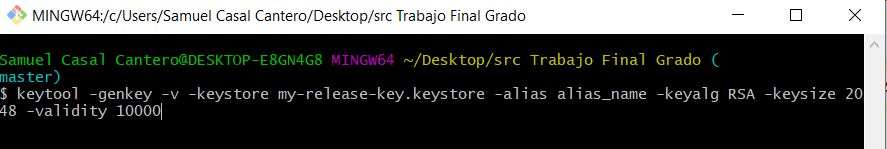
\includegraphics[width=1.0\textwidth]{/techprog/keysnakecommand}
			\caption{Comando generar clave keyStore}
			\label{fig:commandkey}
		\end{figure}	 
	\end{itemize}
	\item \textbf{assets}: directorio que contiene los activos de imágenes y audio de la aplicación. 
	\item \textbf{data/menu-opt.json}: fichero \emph{json} con la estructura del menú \emph{drawer}, con los nombres de ruta, nombre de icono y nombre de la página. 
	\item \textbf{docs/latex}: memoria y anexos del trabajo final de grado.
	\item \textbf{lib}: contiene los ficheros que se compilan para crear la aplicación. La estructura interna de directorios es la siguiente:
	\begin{itemize}
		\item \textbf{main.dart}: fichero principal del que cuelga toda la aplicación.
		\item \textbf{models}: contiene los modelos para crear las instancias de los objetos de la base de datos.
		\item \textbf{pages}: cada una de las interfaces o páginas de la aplicación.
		\item \textbf{providers}: proveedores de algunos servicios internos.
		\item \textbf{routes}: rutas de la aplicación.
		\item \textbf{services}: instancias a los servicios externos de la aplicación.
		\item \textbf{utils}: utilidades.
		\item \textbf{widgets}: elementos gráficos reutilizables.
		 
	\end{itemize}
\end{itemize}
\end{itemize}

%% MANUAL DEL PROGRAMADOR
\section{Manual del programador}
Este manual del programador tiene como objetivo ayudar a las personas futuras que estén interesadas en la continuación del proyecto, o simplemente que tengan ganas de aprender como se ha realizado. Para ello debemos de realizar las instalaciones de las siguientes herramientas:

\begin{itemize}
	\tightlist
	\item Flutter.
	\item Android Studio.
	\item Visual Studio Code.
	\item Git.
\end{itemize}

\subsection{Flutter:}
Es un SDK de código abierto creado por Google. Ofrece la versatilidad de crear aplicaciones móviles tanto como para \emph{iOS} y \emph{Android}, pero también para el entorno web. Internamente el lenguaje de programación es Dart.js, un \emph{framework}, que también es \emph{Open Source} desarrollado por Google, ya que pretende mejorar algunas de las carencias que tiene \emph{javascript}.

Para la instalación de Flutter debemos de ir a su \href{https://flutter.dev/docs/get-started/install}{web oficial} y descargarlo, dependiendo del sistema operativo que tengamos usaremos una versión u otra. (v.17.5 \emph{stable}).

Al descomprimir el fichero nos daremos cuenta de que tenemos un directorio (no ejecutables), por lo que debemos de dejar este en un lugar en concreto para después añadirlo a las variables de usuario. En mi caso yo lo deje en la siguiente ruta de mi ordenador personal C:$\backslash$src$\backslash$flutter.

Una vez tengamos el paso anterior debemos de actualizar las variables de usuario, apuntando al directorio bin de la ruta anterior, como vemos en la siguiente imagen:

\imagen{techprog/variablesEntorno.jpg}{Variables entorno}

\subsection{Android Studio:}
Es el IDE oficial de Google, que remplaza a Eclipse, basado en \emph{IntelliJ IDEA}, publicado de manera gratuita con Licencia Apache 2.0.

En nuestro caso, no programaremos en este IDE, ya que es complicado trabajar con Flutter directamente, solo lo vamos a utilizar para la creación de las máquinas virtuales para emular el sistema operativo Android. Por lo que descargamos de la \href{https://developer.android.com/studio}{web oficial Android Studio} e instalamos.

Una vez lo tengamos instalado creamos las máquinas virtuales, para ello nos vamos a la barra de herramientas Tools>AVD manager y creamos las que sean necesarias, en mi caso tengo dos, con Andorid R, que es la versión 10 de sistema operativo, ya que es la última estable que nos ofrece el IDE.
\imagen{techprog/vm.jpg}{Máquinas virtuales}

\subsection{Visual Studio Code:}
Es el editor de código creado por Microsoft, permite mucha versatilidad y es eficiente para la edición del código en flutter. Es de código abierto bajo la licencia MIT.

Lo podemos descargar de la \href{https://code.visualstudio.com/}{web VS Code}.

Una vez lo tengamos instalado, procedemos a instalar los siguiente \emph{Snippets} que nos ayudan a la creación del código, ya que son como los atajos de teclado. En cada uno de los enlaces, podemos ver una descripción de que es lo que hace cada una de estas herramientas:

\begin{itemize}
	\tightlist
	\item \href{https://marketplace.visualstudio.com/items?itemName=Nash.awesome-flutter-snippets}{Awesome Flutter Snippets}. Apache 2.0.
	\item \href{https://marketplace.visualstudio.com/items?itemName=CoenraadS.bracket-pair-colorizer-2}{Bracket Pair Colorizer 2}. MIT License.
	\item \href{https://marketplace.visualstudio.com/items?itemName=Dart-Code.dart-code}{Dart}. MIT License.
	\item \href{https://marketplace.visualstudio.com/items?itemName=Dart-Code.flutter}{Flutter}. MIT License.
	
\end{itemize}

\section{Compilación, instalación y ejecución del proyecto}

\section{Pruebas del sistema}

	\apendice{Documentación de usuario}

\section{Introducción}
En este apartado se recoge todo lo que un usuario necesita conocer para poder ejecutar la aplicación en su teléfono móvil Android personal y los requisitos mínimos necesarios.

\section{Requisitos de usuarios}
Los requerimientos necesarios para poder ejecutar la aplicación en el teléfono son:
\begin{itemize}
	\tightlist
	\item
	Disponer de un terminal que al menos tenga la versión de Android en \emph{Lollipop}, ya que esta cuenta con el SDK mínimo con el que se ha desarrollado la aplicación, siendo este el 21~\cite{wiki:versionAndroid}.
	\item
	Es necesario disponer de conexión a Internet, tanto como para bajarse la aplicación en \emph{Store}, como para usar los servicios, ya que es necesario logearse con \emph{Google}
	\item La clasificación de contenido, es PEGI 3~\cite{wiki:pegi}. 
	\item En el caso de que la descarga se realice mediante la tienda oficial, los países para los que la aplicación está disponible son: España, Francia, Portugal e Irlanda. En el caso de que no sea así, será necesario descargar desde Github, como se explica en la página~\pageref{descargaGit}.
\end{itemize}

\section{Instalación}
La instalación se puede hacer a través de dos métodos diferentes:

\subsection{GitHub:}\label{descargaGit}
Desde el repositorio donde está el proyecto en el apartado de las \emph{releases}~\cite{github:releases}, podemos encontrar la última de las versiones compiladas, con el fin de descargarla.

Al ser una aplicación de orígenes desconocidos debemos permitir dando permisos de la siguiente manera:
\begin{enumerate}
	\tightlist
	\item Ir a los ajustes del terminal.
	\item Apartado de privacidad o seguridad.
	\item Activar el \emph{slider} de `Orígenes desconocidos''.
	\item Ejecutar el fichero .apk que acabamos de descargar.
	\item Instalar y abrir la aplicación.
\end{enumerate}

\subsection{Play Store:}
La manera más cómoda de hacerlo, es dirigirse \href{https://play.google.com/store/apps/details?id=com.ubu.flutter_snake}{Flutter games}, que es el enlace de descarga para dispositivos móviles Android. La versión disponible es la 6, ya que he tenido que realizar varias pruebas, con el fin de validar la disponibilidad, por eso el número que tiene.



\imagen{manual/tienda.jpg}{Tienda con el proyecto}

El proceso de instalación es simple, solo tenemos que dar al botón de instalar. En el caso de que nos encontremos en el navegador web, nos deja elegir el dispositivo que tenemos vinculado a nuestra cuenta de \emph{Google}. Si por otra parte nos encontramos desde el terminal, se instalará sin ningún problema.

En el caso de que se lancen nuevas versiones del producto, las actualizaciones se realizarán de forma automática.

\section{Manual del usuario}



	
	
	\bibliographystyle{plain}
	\bibliography{bibliografiaAnexos}
	
\end{document}